% ------------------------------------------------------------------------ %
% !TEX encoding = UTF-8 Unicode
% !TEX TS-program = pdflatex
% !TEX root = ../Tesi.tex
% !TeX spellcheck = en_US
% ------------------------------------------------------------------------ %
%
% ------------------------------------------------------------------------ %
% 	PROPOSED SOLUTION
% ------------------------------------------------------------------------ %
%
\chapter{Proposed Solution}
%
\label{cap:proposedsolution}
%
% ------------------------------------------------------------------------ %
%
\par In this chapter the development of the solution will be reported step by step, with a full use case. The chapter starts with a list of similar solutions already developed, highlighting the differences between them and my thesis work. The remaining part is composed of tree mains sections: the first explains the choice of the network, the architecture, the naming service, etc. It lays the foundations for the second part: the definition of the Liquid Android middleware, or better the structure of what will do the magic: intercept, encapsulate, spread, and generate distributed intents in the network so made. The two parts are closely related, therefore their relation was taken into account when I made my choice.\\
The real implementation of the valid solution is left for the next chapter.
%

\section{Existing Solutions }
Android distributed systems already exists as specific purposes application to be installed on multiple devices, what it is different to the aim of this thesis work is that these application are closed source projects that can not be reused to build other purposes systems and there is not a coherent framework, library or API to be used to easily build such systems.
I want to give some examples pointing out the nice features have this native distributed Android systems.
\subsection{Boincoid and HTC Power to Give}
Boincoid and HTC Power to Give are Android application which aim is  to exploit Android devices computation power to contribute to scientific discoveries by doing some task. The common idea is to have an Android distributed supercomputer which can handle heavy task and compute tons of data for larger purposes.\\
BOINC is an open-source software platform for computing using volunteered resources \cite{boinc2017open}. It is a program that lets you donate your idle computer time to science projects. Boincoid is a port of the BOINC platform to the Android operating system. The result is an Android BOINC client that behaves exactly like the original one.\\
HTC Power to give is very similar to Boincoid, it is a \textit{CSR (Corporate Social Responsibility)} initiative from HTC that has been jointly developed with Dr. David Anderson at University of California, Berkeley. Using the HTC Power To Give, owners of Android OS smartphones can choose to ‘give back’ by supporting key research projects around the world. Scientific research often requires a vast amount of processing power for data modeling and analysis. HTC Power To Give, supported by the world’s largest single distributed volunteer computing platform BOINC, lets users donate their unused smartphone computing power to science programmes across diverse fields as astronomy, environment, medicine and physics \cite{htc2017power}.
 
\subsection{Plex for Android}
Plex platform is a great, maybe the best, media content streaming distributed system platform. It is mainly composed of two components, the media server, and a client with which enjoy the contents.
\begin{figure}[h]
	\centering
	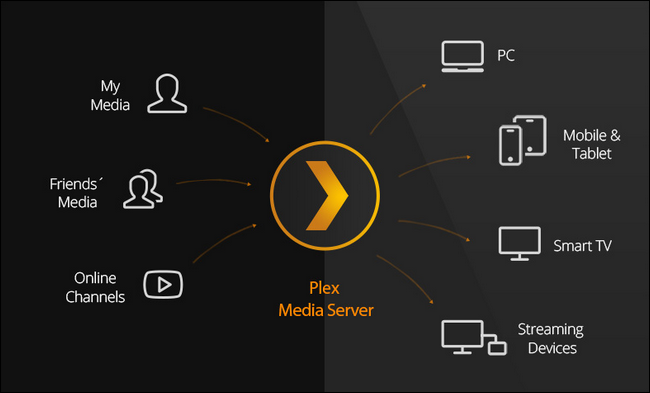
\includegraphics[width=.8\textwidth]{plex}
	\caption{Plex Platform}
	\label{fig:4.1}
\end{figure}
The Plex Media Server either running on Windows, macOS, Linux, FreeBSD or a NAS which organizes audio (music) and visual (photos and videos) content from personal media libraries and streams it to their player counterparts.
The players can either be the Plex Apps available for mobile devices, smart TVs, and streaming boxes, or the web UI of the Plex Media Server called Plex Web App, or the old Plex player called Plex Home Theater.\\
In particular Plex for Android application can connect to the media server to play its content and in addition it can search for Plex players in a LAN and send streamed content such as videos, movies or photo, to another player that can be also an Android device. In this way the Android Plex application client can behave like the Liquid Android system i want to develop. It can send a sort of \textit{Android intent}, to reproduce a media, from one device to another, and then it can send commands such as pause, rewind, forward and so on. The limits of such a system are that it is possible to send, and play, only multimedia contents, and only to devices which have the Plex app activity in foreground on the device.

\subsection{Goolgle Home and Cast API}
Google itself provides an application to control and send contents form an Android device, to some special devices in home network. \textit{Google Home} is an Android application which can find, setup, manage and control, Google's home devices like the \textit{Google Chromecast}. In this way is easy to setup and control and Android distributed system in which user can sent multimedia contents and command to the Google Home devices in the LAN. For these reason Google provides a development library, included in the Android framework, called \textit{Cast API} with which it is easy, for a developer, to build applications that can send multimedia streams to other Google devices specifically built for these purposes.\\
Also in this case the limitation is the kind of content, only multimedia, and also the type of devices involved which are limited number of special purposes devices.

\subsection{DroidMote and Remote control systems }
If we consider the possibility to control remote devices in a LAN, there are actually many different kind of applications that can do that also in an Android environment.
DroidMote is probably the most complete application to control remotely an Android device from another one. It is composed by two parts, the server, to be installed in the device to be controlled, and the client, to be installed in the one which controls. With this application is possible to control entirely the device running the server component: is it possible to open applications, perform tasks, open system settings and so on.\\
These kind of systems are capable to generate local intents in remote devices over a LAN but in a completely different way from I want to develop the solution to the given problem. In this case the \textit{controller} is explicitly controlling the remote device as it is using only the \textit{controlled} one. These systems are solution only to the problem of remote control, they can not exploit distributed Android devices computation power, in fact in an environment like this Android devices are not cooperating to perform task but one of them is only controlling another one.
\section{General Idea}
\par To better explain what I consider solution for my work it is important to
understand the playground to my work. As said in the previous chapter, \ref{cap:probanalysis}, I
am trying to extend the Android operating system by adding some functionalities to make it similar to a distributed OS, without the need of rooting it or change its standard working mechanism and components, staying in the 7th layer of the ISO/OSI stack , the application layer. Using already developed and operating tools, and respecting all the above listed constraints I am going to make mobile devices in a LAN network communicate and cooperate like they were using a single coherent distributed operating system.
In order to understand what is needed and how it is possible to solve the problem
it is fundamental to understand the type of stack and the network structure
we have to face, and standard Android working principle, in particular the intent resolution mechanism already described in \figurename~\ref{fig:2.4}.\\
Only having clear in mind the problem and its structure it is possible to find the best possible solution. In particular it is possible to decompose the main problem in some sub-problems, which can be understood as general steps in doing similar works of extending a mobile OS to become a distributed OS:
\begin{itemize}
	\item Network architecture, that is the structure and the classification of the nodes involved in the distributed system. As previously said it has to be as reliable  as possible and allow dynamic connection due to the fact that nodes are mobile devices and can be easily moved in and out the network range.
	\item Communication model, that is the way in which involved actors perform the communication. It has to be compliant to M2M, and possibly to H2M communication, and as lightweight as possible to allow fast exchange of messages and data between the network nodes.
	\item Data model, as discussed before in the chapter \ref{cap:statoarte}, when building distributed systems it is also important to guarantee that data are managed correctly by adopting a consistency policy.
\end{itemize}
It is also necessary to identity the main actor involved in the problem, they are mainly two:
\begin{itemize}
	\item Server application, it is the main actor of this thesis work, it must be an Android application which once installed on a compatible Android device can receive resolve and forward Android intents. It contains the logic and the controllers needed to handle the network structure, find other devices in the network, send and receive messages. It is responsible of resolving all the three sub-problems described above. The server application has also the double function of receiving a message from the network and translate it in a local intent to be resolved by the Android operating system, but also it can act as a client by forwarding a received intent from a third party client application to another server in the net, by encapsulating the intent in a network message.
	\item Clients, can be applications developed in several ways, they are those which are asking to the so called servers to complete task for them. In this case clients could be any kind of third party Android application installed in the device, also running the server component, generating implicit Android intents that need to be resolved by the OS. 
\end{itemize}
Once defined the main actors of the problem I am facing, the next step is to understand how they can interact and communicate. As previously described defining the problematic scenarios in the chapter \ref{cap:probanalysis}, the Liquid Android middleware in the best case would be a system service which users can control to distribute intents in the local network by using the WiFi chip of the devices.
 \begin{figure}[h]
	\centering
	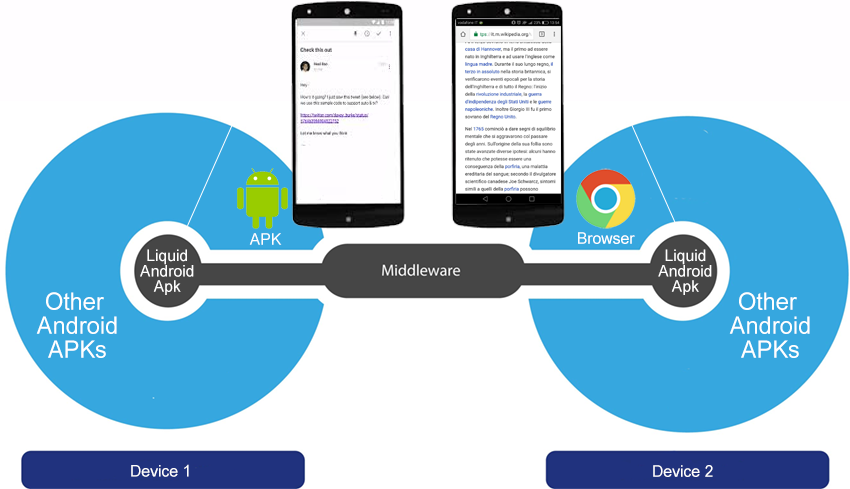
\includegraphics[width=.9\textwidth]{esempio1}
	\caption{Liquid Android working example}
	\label{fig:4.2}
\end{figure}
The \figurename~\ref{fig:4.2} shows exactly how the middleware is supposed to work. In the figure the two devices are both supposed to be connected to the same local network \textit{(they are under the same WiFi access point)} and they are executing any standard Android OS version starting from 4.4 KitKat \textit{(API level 19)}. The so called, in the picture, \textit{Device 1} is executing a third party application activity \textit{(a client)}  which contains a valid clickable URL link. By clicking a link, typically, Android applications generate an implicit intent asking to the OS to open and show the page linked by the URL. Usually, in the absence of other applications capable of solving this kind of implicit intent, the process ends with the opening of a browser in the same device, which opens the URL in one of its activities. In this case the Liquid Android application server, installed on both devices, should to tell the OS that it can handle that implicit intent, find the other devices in the net, in this case the so called \textit{Device 2}, le the user choose with which device complete the task, convert the intent in a network message and send it to that device. Once the message arrived to the \textit{Device 2} the Liquid Android middleware server application is responsible to translate again the received message into the starting implicit intent sent by the \textit{Device 1} and to start the very same resolution mechanism for that intent by its own Android operating system, which should end by the opening of a browser activity to view the page.\\
It is clear that a solution for this scenario would be also, once implemented, a solution for the second problematic scenario proposed in \ref{devAPI}. In fact we can consider the development of an API to build native Android distributed systems as a sub problem of the first one, already described above and in \ref{middlewarescenario}. The implemented version of the general solution could be also used as a library to implement special purposes similar systems by simply extending my framework and including its implemented Java classes in other Android applications projects. For these reasons in developing the solution I will try to make it as clear as possible, and to parametrize as far as possible the settings variable of my framework to make it easily extensible and ready to use buy other Android developers.\\
I would like now to list the goals that my work has to match, in order to be a valid proposal for solving the given problem. These goals are not to be intended as set in stone, they are the general motivation that leads to construct a prototype of the proposed software architecture. According to my thoughts during the development, it is possible to identify the following goals:
\begin{itemize}
	\item The middleware must work without any proprietary application: it has to interface itself to the upper layer without installing any other application of any vendor in the owned device. It must be completely neutral to the market, it must work with any version of the Android operating system starting from the API level 19, also with Android customized versions developed by device maker like Samsung, LG, Huawei and any other brand. It is the fundamental requirement to create heterogeneous applications and to separate the various closed solutions of today and an open solution for everyone in the future.
	\item The middleware has to simplify the life of the developer, he should not have to worry too much about the substrates, he should be able to fast prototype. The developer should see my framework as help for his work. The idea is to provide a ready to use service, with which it is possible create new application by exploiting it.
	\item The middleware should offer the user the possibility to access directly to other devices in the network without the need of configure anything. Users, once installed the middleware should use its functionalities of receiving/forwarding intents in a transparent way, in the same way they use other applications and with the same mechanism they learned by using the standard Android operating system.
\end{itemize}
The next sections contain all the steps necessary to have a full working system.
Firstly I would solve the, let me call it \textit{general theoretical problem} by dividing it as discussed above and providing the solution for each of them, taking into account also the data management scenario. Then I would like to present the structure of the development API, while the actual implementation of the working Liquid Android application is left for the next chapter with some working tests and a deep component analysis.



\section{Theoretical solution, extending the Android OS}
\par In this section i will perform an in depth analysis of the possible solution to the given problem: how I can extend the Android OS providing it distributed functionalities.
\subsection{Network Architecture}
The first step while creating a distributed system is to define the networking architecture, in particular I must define the kind of nodes involved in the system and the way in which they interact, what they can do, which operation they can perform and in which way. As mentioned earlier the network architecture of the system must fulfill the following requirements:
\begin{itemize}
 \item \textit{dynamicity}, it must allow any device to perform the dynamic connection, and also disconnection, to the distributed system at any time, since the nodes of the network are mainly mobile devices and they can be moved easily. Nodes can \textit{JOIN} and \textit{LEAVE} every time, and the network must accommodate them automatically.
  \item \textit{simplicity}, the network must be as simple as possible, it should not need any particular configuration on the nodes to \textit{JOIN}. Any node should perform other nodes \textit{DISCOVERY} in the network in a easy way without the need to know them a priori.
 \item \textit{reliability and security}, are important non functional requirements in such a system. I want to make the network reliable and secure as much as possible by the adoption of standard software engineering techniques.
\end{itemize}
The network architecture that fits better all the requirements listed above is certainly a P2P network. As seen in \ref{P2P}, in peer-ro-peer networks there is not a clear distinction between clients and servers, in fact a peer-to-peer network is designed around the notion of equal peer nodes simultaneously functioning as both "clients" and "servers" to the other nodes on the network.

\begin{figure}[h]
\centering
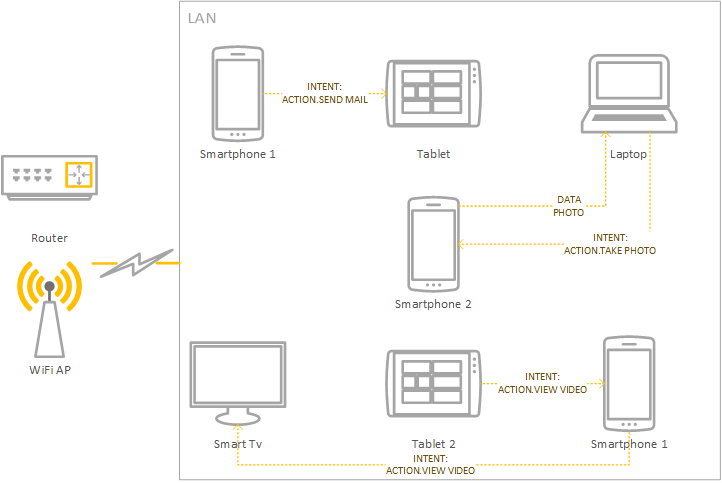
\includegraphics[width=.9\textwidth]{P2Pnetwork}
\caption{P2P Liquid Android network example}
\label{fig:4.3}
\end{figure}
I think that an \textit{unstructured P2P architecture} is the best choice for my system due to the fact that it do not impose a particular structure on the overlay network by design and data is still exchanged directly over the underlying TCP/IP network, so at the application layer peers are able to communicate with each other directly, via the logical overlay links. In \figurename~\ref{fig:4.3} there is an example of my architecture in which different devices are in range under the same local network and they can communicate sending intents and data.\\
To obtain this kind of structure, and let it change dynamically depending on the devices in range, I need to equip the devices with a \textit{network service}. In computer networking, a network service is an application running at the network application layer and above, that provides data storage, manipulation, presentation, communication or other capability which, in this case will be used in combination with a peer-to-peer architecture based on the application layer network protocols. Different services use different packet transmission techniques. In general, packets that must get through in the correct order, without loss, use TCP, whereas real time services where later packets are more important than older packets use UDP. For example, file transfer requires complete accuracy and so is normally done using TCP, and audio conferencing is frequently done via UDP, where momentary glitches may not be noticed. In this case I will adopt the TCP transport layer because I need to transfer packets in reliable way, as much as possible, and also avoid network congestions, the UDP protocol in fact lacks built-in network congestion avoidance while TCP has it.\\
To fulfill the above listed requirements of dynamicity and simplicity the right approach should be the Zeroconf one, already discussed in \ref{zeroconf}. Using a Zeroconf implementation to register and discover the service in the LAN will let the node to connect dynamically and in a easy way to the distributed system. The three main operation a node can perform are:
\begin{itemize}
	\item \textit{JOIN}, to join the system a node must activate the network service, it must provide an internal endpoint for sending or receiving data in the computer network. The best abstraction to do that is to open a socket, as seen in \ref{socket}. In particular, a TCP socket is characterized by two main parameters: the \textit{IP} and the service \textit{PORT}. In my system the TCP socket is a great choice because, as already stated, it is a network abstraction and it can be used to let communicate heterogeneous devices and can be implemented in several different ways using basically any development language. By knowing the couple of variable of the network service another device can send message, streams and so on, to it through the TCP socket.  Since mobile devices changes frequently their connections variables, because of their nature to be easily moved from one place to another, we need a system that can identify them dynamically. The name of the service and the chosen transport layer can be established once for all and they can never change. In this environment Zeroconf provides service registration and discovery. By registering the service name, port, and transport layer the node can be found in the LAN by other nodes looking for that kind of service. In this way nodes do not need to know, a priori, the two variables, IP and PORT of any node in the network, to communicate with each other, they, indeed, need only to know the service name and the chosen transport layer to find other nodes in the network.
	\lstinputlisting[language=Java , caption=Zerconf registration example , label=code:4.1]{Codici/registerservice.java}
	The snippet of code \ref{code:4.1} is an example of how in Android it is possible to register a service using the Zeroconf approach. Once registered the service Zeroconf provides name resolution functionalities to discover other nodes and then connect to them to start the communication.
	\item \textit{LEAVE}, I want that a node can decide whether join or leave the network at any time. To leave the network a node should only unregister the service registered using Zeroconf and then close the socket to avoid accidental or malicious connections.
	\item \textit{SEARCH}, since the network is dynamic, it is necessary to determine how the nodes, once the service has registered, can search for and find other nodes. As already mentioned describing the \textit{JOIN} operation Zeroconf also provide the network service discovery and the naming resolution mechanism. In this case Zeroconf uses a \textit{Domain Name System (DNS) based Service Discovery}, the so called \textit{DNS-DS}. DNS-SD allows clients to discover a named list of service instances, given a service type, and to resolve those services to \textit{hostnames} using standard DNS queries. The specification is compatible with existing \textit{unicast DNS} server and client software, but works equally well with \textit{multicast DNS (mDNS)} in a zero-configuration environment. Each service instance is described using a \textit{DNS SRV} and \textit{DNS TXT} record. A client discovers the list of available instances for a given service type by querying the \textit{DNS PTR} record of that service type's name; the server returns zero or more names of the form "<Service>.<Domain>", each corresponding to a SRV/TXT record pair. The SRV record resolves to the domain name providing the instance, while the TXT can contain service-specific configuration parameter. Once completed the resolution process the node which started it to find other nodes in the network, knows any couple of IP/PORT of their open sockets and can connect to them to exchange messages or transfer data.
\end{itemize}
Given the network structure security is obviously a non functional requirement in building my system, but since my entire middleware, once connected, will allow to send and execute any kind of task, in the form of implicit intents, to each device involved I need to make some considerations about the security of such a system. The security of my system is highly influenced by the underlying physical network, if the LAN access is secured and protected my system will be, indeed, enough secure. The network should be protected using a firewall and the service ports used by the device involved in the system should not be accessible from the outside of the LAN. Moreover the WiFi should be protected using a strong password and a secure and updated access protocol like the\textit{WPA2}. Furthermore, I want that users of my system are aware of the fact that it is running, so once the service is activated users will be alerted by a notification in the appropriate Android notification area.
 
 \subsection{Communication Model}
 Once the network is up the second step is let the device communicate to cooperate giving, to the final users, the feeling that they are working with a single big distributed operating system. To achieve this goal, as already explained several times, my system is supposed to intercept implicit intents, let the user select a target device, or a group of them, to perform the task, send it and once arrived perform it in the selected device or group devices. With TCP sockets it very easy to exchange messages between networked devices, so it is equally easy to understand why I have chosen a message oriented structure as the communication model, briefly presented in \ref{messageo}, for my system. Furthermore, as already stated with the \tablename~\ref{tab:comp} such a model gives me more freedom of choice regarding certain characteristics that the system must have, I want the communication is:
 \begin{itemize}
	\item \textit{concurrent}, in the original Android OS when an intent resolution mechanism is started by any other component of the system, for example an application activity, the OS stops its execution to perform, in foreground, the task the intent contains. I want to leave unchanged this kind of mechanism in my system, so when a, let me call it, \textit{distributed intent} arrives from the socket, the operating system must treat it exactly as if it were a \textit{local intent} and execute it in the same way it does with other intents. The arrival of a new distributed intent from another device is the event which triggers the standard OS resolution technique by suspending any other operation. I want the network listen and accepts messages with distributed intents to solve at any moment, in a fully concurrent way, so the last intent is triggered the first it is resolved and executed in a \textit{LIFO}, last in first out, way like in a stack structure.
	\item \textit{asynchronous}, the standard intent resolution mechanism, like many other in the Android operating system, is mainly asynchronous. When an implicit intent is triggered it will be performed without knowing, a priori, what application will execute the task and how. To be more clear, for example when an application ask the OS to open a map of a place, the application which started the process do no need to know if the system completed the task and with which results. I want that my system do not need to change this behavior, if an operation need to be performed the intent is triggered and the OS reacts as usual without the need to send back acknowledgment messages \text{ACKs}. When it is necessary to synchronize the communication among the various components involved when an implicit intent is triggered Android provides a mechanism, using the system function \textit{startActivityForResult(intent)}, to send the result back to the caller. I intend to keep the same mechanism also when dealing with distributed intents, but I want to maintain an asynchronous approach also in this case, the caller could continue its execution without waiting for the results and then, once done, receive back the response, in the form of another distributed intent, from the called. I will give further details of this case when presenting the kind of messages can be sent using my system and the data model solution part.
 \end{itemize}

Now the difficult part is establish how intents can be sent through the sockets and which kind of messages my system can send and then handle to perform various kind of tasks.\\
The next step, hence, is to find a way to send the intents from a device to another without loosing information and once they are arrived to be executed like they were local intents. To do this job it is necessary to analyze in dept what an intent is in Android and what it can contain.\\
As showed in the chapter \ref{cap:statoarte} in \ref{intents} intents are the way in which standard Android framework's components communicate among each other, and they also represent the abstraction of actions to be performed by Android applications. In the Android developer framework an intent is implemented as a Java Class containing the information and data to perform the task. An intent is an abstract description of an operation to be performed. It can be used in various ways: with \textit{startActivity} to launch an Activity, with \textit{broadcastIntent} to send it to any interested \textit{BroadcastReceiver} components, and  with \textit{startService(Intent)} or \textit{bindService(Intent, ServiceConnection, int)} to communicate with a background Service. However its most significant use is in the launching of activities, where it can be thought of as the glue between activities. It is basically a passive data structure holding an abstract description of an action to be performed \cite{android2017intent}.\\
Every implicit intent is characterized, mainly, by an \textit{ACTION}, \textit{DATA} and a bundle of \textit{EXTRAS}.
\begin{table}[h]
	%
	\caption{Intent Structure}
	%
	\label{tab:intent}
	%
	\centering
	\begin{center}
	
	%
	\begin{tabular}{>{\centering\arraybackslash} m{0.15\textwidth}p{0.4\textwidth}p{0.4\textwidth}}
		%
		
		\toprule
		%
		\centering\textbf{Attribute} & \centering\textbf{Description}  &\begin{minipage}[t]{0.4\textwidth}
			\centering
		\textbf{Examples}
		\end{minipage} \\
		%
		\midrule
		%
		\centering\textit{ACTION} & \begin{minipage}[t]{0.4\textwidth}
			\centering
		The general action to be\\ performed.
		\end{minipage} & \begin{minipage}[t]{0.4\textwidth}
		\centering
		ACTION\_VIEW\\ACTION\_EDIT
		\end{minipage}\\ %fine riga tabella
		&&\\
		\centering\textit{DATA} & \begin{minipage}[t]{0.4\textwidth}
			\centering
		The data to operate on,\\expressed as a Uri.
		\end{minipage} &
		\begin{minipage}[t]{0.4\textwidth}
			\centering
		content://contacts/people/1 \\ tel:123
		\end{minipage}\\  %fine riga tabella
		&&\\
		\centering\textit{CATEGORY} & \begin{minipage}[t]{0.4\textwidth}
			\centering
			Gives additional information\\about the action to execute.
		\end{minipage} &
		\begin{minipage}[t]{0.4\textwidth}
			\centering
			 CATEGORY\_LAUNCHER \\  CATEGORY\_ALTERNATIVE
		\end{minipage}\\  %fine riga tabella
		&&\\
		\centering\textit{TYPE} & \begin{minipage}[t]{0.4\textwidth}
			\centering
			Specifies an explicit type \\(a MIME type) of the intent data. Normally the type is inferred\\ from the data itself. 
		\end{minipage} &
		\begin{minipage}[t]{0.4\textwidth}
			\centering
			type */*
		\end{minipage}\\  %fine riga tabella
		&&\\
		\centering\textit{EXTRAS} & \begin{minipage}[t]{0.4\textwidth}
			\centering
		This is a Bundle of any additional information. This can be used to provide extended information to the component.
		\end{minipage} &
		\begin{minipage}[t]{0.4\textwidth}
			\centering
			EXTRA\_TEXT\\
			EXTRA\_TITLE
		\end{minipage}\\  %fine riga tabella
	
		\bottomrule
		%
	\end{tabular}
\end{center}
	%
\end{table}
The \tablename~\ref{tab:intent} explains in depth what an intent could contain, of course there are many types of action, data, categories and extra that are not reported here for reasons of brevity but that can be found in \cite{android2017intent}. The real problem, for the purposes of my system, is that the Android intent Java Class can no be serialized,automatically and send through the socket as it is. In computer science serialization is the process of translating data structures or object state into a format that can be stored, or transmitted across a network connection link, and reconstructed later in the same or another computer environment. When the resulting series of bits is reread according to the serialization format, it can be used to create a semantically identical clone of the original object \cite{marshall2015c++}. In a Java environment, like the Android one, Java Classes that implements the \textit{Serializable interface} can be automatically serialized, by the environment itself, and sent through a socket  and then automatically deserialized to reconstruct the original sent object by the receiver, but as already told the intent Class does not implement this functionality. I need therefore to find a way to do this process in a fully functional and also efficient way. There are, actually, many alternatives to accomplish this objective. For example I could generate a new Java Object, containing all the intent attributes, that implements the Java Serializable interface, convert intents to this new Object and then let Java perform its automatic serialization/serialization. As an alternative I could generate some kind of semi-structured data, using a well know, let me call it \textit{container language}, such as JSON or XML, which can be easily sent, as a string, over the socket and then parsed to rebuild the original Java Object.\\
Since the effort required to develop one of the two solution, presented above as examples, is practically the same, I decided to opt for the second alternative, using a JSON structure, because it has substantial advantages.\\
JSON (JavaScript Object Notation) is a lightweight data-interchange format. It is easy for humans to read and write. It is easy for machines to parse and generate. It is based on a subset of the JavaScript Programming Language, it is completely language independent. These properties make JSON an ideal data-interchange
language \cite{w3c2007introducing}.\\
It is based mainly on two types of structures:
\begin{itemize}
	\item Key/Value pair set: it can be considered an object of an Object Oriented programming language,
	\item Collection of elements: it can be considered an array of Objects.
\end{itemize}
 \subsection{Data management Model}

 



%
% -----------------------------END--------------------------------- %